\documentclass{article}
\author{RustColeone}
\usepackage{amsmath}
\usepackage{amsfonts}
\usepackage{enumitem}
\usepackage{titling}
\usepackage{aligned-overset}
\usepackage{tikz}
\usepackage{hyperref}
%\setlength{\droptitle}{-12em}
\title{ECE, Signal Processing}
\setlength{\parindent}{0pt}
\newlength\tindent
\setlength{\tindent}{\parindent}
\setlength{\parindent}{0pt}
\renewcommand{\indent}{\hspace*{\tindent}}

\begin{document}
\maketitle
\newpage
\tableofcontents
\newpage
\section{Sinusoidal Signals}
    \begin{enumerate}
        \item Sinusoidal signals are the basic building blocks in the theory of signals \& systems
        \item Arise as soutions to differential equations that through the laws of physics, describe common physical phenomena
    \end{enumerate}
    \subsection{Mathematical Formula}
    let a signal be $s(t)$, where t represents the time t of a given time, we have:
    \begin{align}
        s(t) &= A cos(2 \pi f_0 + \phi)
    \end{align}
    A linear function of time t, in which \textbf{A is the amplitude} that scales the cosine signal in y dimention, since
    \begin{align}
        -1 \leq cos(x) \leq 1 \text{for all } x, s(t) \in [-A, +A]
    \end{align}

    \textbf{$\phi$ is the phase in (rad)} that determines the time locations of the maxima and minima of $s(t)$\\\indent

    eg: $\phi = 0 \implies s(0) = Acos(0) = A$, so $s(t)$ has a local maxima at 0

    if $\phi != 0 \implies s(0) = Acos(\phi)$, which is not necessary A\\\indent
    
    Finding Maximum of the signal after t = 0
    \begin{align}
        Acos(2 \pi f_0 t + \phi) = A &\equiv cos(2 \pi f_0 t + \phi) = 1 \\
        2 \pi f_0 t + \phi &= 2 k pi \\
        t &= \frac{2 k pi - \phi}{2 \pi f_0}, \text{ } k \in \mathbb{Z}
    \end{align}

    \textbf{$f_0$ is the frequency in (Hz)}, determines the rate the signal oscillates
    
    \begin{align}
        \text{Period } T_0 &= \frac{1}{f_0}
    \end{align}
    \subsection{Periodic Signals}
    A periodic signal persists for an infinity amount of time, and will always output the same waveform in any integer multiples of periods

    \begin{align}
        s(t + T_0) &= s(t + T_0), \text{ for all t}
    \end{align}
    
    We can express $\phi$ as
    \begin{align}
        \phi &= 2 k \pi + \phi_0, k \in \mathbb{{z}}, \phi_0 \in [-\pi, \pi]
    \end{align}

    if $f_0 = 0$, for all values of $A cos(\phi)$ is a constant, hence a DC signal
    
    We can ecpress any arbitrary sinusoidal signal as a linear combination of the two pure sinusoidal signals:
    \begin{align}
        s(t) &= R \times cos(2 \pi f_0 t + \phi)\\
        s(t) &= A \times cos(s \pi f_0 t) + B \times sin(s \pi f_0 t)
    \end{align}
    where $A = R cos(\phi)$ and $B = R sin(\phi)$\\
    Using the formulae:
    \begin{align}
        sin(A \pm B) &\equiv sin(A)cos(B) \pm cos(A)sin(B)\\
        cos(A \pm B) &\equiv cos(A)cos(B) \mp sin(A)sin(B)\\
        tan(A \pm B) &\equiv \frac{tan(A) \pm tan(B)}{1 \mp Atan(B)}\\
        sin(3A) &\equiv 3sin(A) - 4sin^3(A)\\
        cos(3A) &\equiv 4cos^3(A) - 3cos(A)\\
        sin(P) + sin(Q) &\equiv  2 sin (\frac{1}{2}(P + Q)) cos (\frac{1}{2}(P - Q))\\
        sin(P) - sin(Q) &\equiv  2 cos (\frac{1}{2}(P + Q)) sin (\frac{1}{2}(P - Q))\\
        cos(P) + cos(Q) &\equiv  2 cos (\frac{1}{2}(P + Q)) cos (\frac{1}{2}(P - Q))\\
        cos(P) - cos(Q) &\equiv -2 sin (\frac{1}{2}(P + Q)) sin (\frac{1}{2}(P - Q))\\
    \end{align}

    \subsection{Harmonics}
    Lets say we have Harmonic Frequencies $f_k, k \in \mathbb{Z}$
    \begin{align}
        x_1(t) &= cos(2 \pi f_1 + \phi)\\
        x_2(t) &= cos(2 \pi f_2 + \phi)\\
        f_k &= k \times f_0, k \in \mathbb{Z}
    \end{align}
    Proof\:Any linear combination of sinusoidal signals of harmonics of some frequency $f_0$ is a periodic signal
    \begin{align}
        \text{For arbitrary } \{A_k\} \{\phi\}\\
        s(t) =& \sum_{k=1}^{N} A_k cos(2 \pi f_0t + \phi_k)\\
        s(t) =& \sum_{k=1}^{N} A_k cos(2 \pi f_0t + \phi_k)\\
        s(t + T_0) =& \sum_{k=1}^{N} A_k cos(2 \pi f_0 t + 2 \pi k + \phi_k)\\
        \text{hence: } s(t + T_0) =& s(t)\\
    \end{align}
    \subsection{Fourier Series}
    We can express any arbitrary periodic signal as a sum of harmonic sinusoids,
    let $x(t) = x(t + T_0)$ be a periodic signal with period $T_0$\\
    Then there exist coefficients:
    \begin{align}
        \{A_k\}_{k = 0}^{\infty}, \{B_k\}_{k = 0}^{\infty}\\
        x(t) &= \frac{A_0}{2} + \sum_{k=0}^{\infty}\left( A_k cos(2 \pi f_0 k t) + B_k sin(2 \pi f_0 k t)\right), \forall t
    \end{align}
    Calculating $\{A_k\}, \{B_k\}$ starting from $x(t)$
    It can be shown that:
    \begin{align}
        A_k &= \frac{2}{T_0} \int_{-0.5T_0}^{0.5T_0} x(t)cos(2\pi kt)dt\\
        B_k &= \frac{2}{T_0} \int_{-0.5T_0}^{0.5T_0} x(t)sin(2\pi kt)dt
    \end{align}

    Fourier synthesis is the reverse process of starting from 
    $\{A_k\}_{k = 0}^{\infty}, \{B_k\}_{k = 0}^{\infty}$ and generates a periodic signal\\\indent

    Equivalent Form:
    \begin{align}
        s(t) &= \frac{A_0}{2} \sum_{k=1}^{\infty} C_k cos(2 \pi f_0t + \phi_k)\\
        \text{where} \nonumber\\
        C_k &= \sqrt{A_k^2 + B_k^2} and \phi_k = tan^{-1}(\frac{B}{A})
    \end{align}

%    \begin{tikzpicture}
%        \draw[->] (-3,0) -- (4.2,0) node[right] {$x$};
%        \draw[->] (0,-3) -- (0,4.2) node[above] {$y$};
%        \foreach \ini [evaluate=\ini as \inieval using 2*\ini] in {0,...,1}
%        \draw[ultra thick,cyan] (\inieval,0) -- ++(0,3) -| (\inieval+1,0) -- (\inieval+2,0);
%        \draw[scale=0.5,domain=-3:3,smooth,variable=\y,red]  plot ({\y*\y},{\y});
%    \end{tikzpicture}

    \subsection{Spectrum}
    Fourier thyrm showed that all periodic signals can be written as an addictive linear combination of sinusoid signals

    The spectrum of a periodic signal is the collection of amplitude, frequency and phase information that allow us to represent the signal as a linear combination
    \begin{enumerate}
        \item Time-domain: need knowledge of $f_0, A_0, \text{ and } \{x(t), t\in[-\frac{T_0}{2},\frac{T_0}{2}]\}$
        \item Frequency-domain: Would require $f_0, A_0, \{C_k\}_{k=1}^{\infty}, \{\phi_k\}_{k=1}^{\infty}$
    \end{enumerate}
    The spectrum is given by the following collection:
    
    \begin{tabular}{ |p{3cm}|p{3cm}|p{3cm}|  }
        \hline
        Frequency & Amplitude & Phase \\
        \hline
        \;\;\;0 & \;\;\;$A_0$ & \;\;\;0\\
        \;\;\;$f_0$ & \;\;\;$C_1$ & \;\;\;$\phi_1$\\
        \;\;\;$2f_0$ & \;\;\;$C_2$ & \;\;\;$\phi_2$\\
        \;\;\;$\;\vdots$ & \;\;\;$\;\vdots$ & \;\;\;$\;\vdots$\\
        \;\;\;$f_0$ & \;\;\;$A_0$ & \;\;\;$\phi_1$\\[1ex]
        \hline
    \end{tabular}
    \subsubsection{Graphical plot of the spectrum}
    \begin{center}
        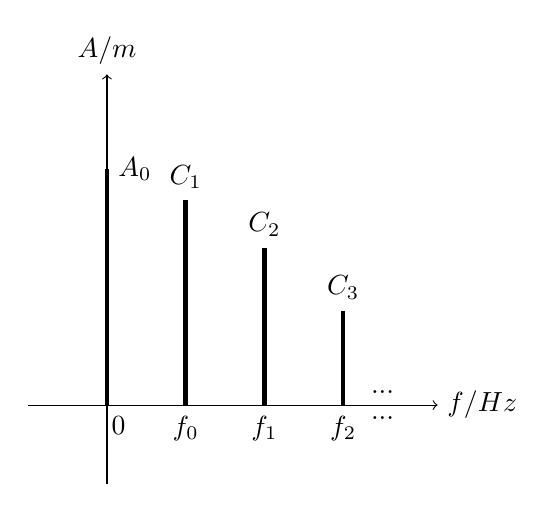
\begin{tikzpicture}
            \draw[->] (-1,0) -- (4.2,0) node[right] {$f/Hz$};
            \draw[->] (0,-1) -- (0,4.2) node[above] {$A/m$};
            \draw[ultra thick, black] (0,0) node[below] {$\;\;\;0$} -- (0,3) node[right] {$A_0$};
            \draw[ultra thick, black] (1,0) node[below] {$f_0$} -- (1,2.6) node[above] {$C_1$};
            \draw[ultra thick, black] (2,0) node[below] {$f_1$} -- (2,2.0) node[above] {$C_2$};
            \draw[ultra thick, black] (3,0) node[below] {$f_2$} -- (3,1.2) node[above] {$C_3$};
            \draw[ultra thick, black] (3.5,0) node[below] {$...$} -- (3.5,0) node[above] {$...$};
        \end{tikzpicture}
    \end{center}
    In which the vertical plots are the spectral lines
    \begin{center}
        $\rightarrow\;$\text{analysis} $\rightarrow$\\
        $\text{Time Domain} \Longleftrightarrow \text{Frequency Domain}$\\
        $\leftarrow$ \text{syntheses}$\;\leftarrow$
    \end{center}

    \subsubsection{Benefits of spectrum}
    \begin{enumerate}
        \item Often time-waveforms are very complicated while spectrun is more straight forward
        \item We can compress data by only storing the important frequencies, shrinking file size (mp3)
        \item Understanding the properties of the signal is often insightful on how to process item
        \begin{itemize}
            \item Think of audio processing, mp3 is a format which removes all frequencies sampled beyond human's limits, also shrinking the file size
            \item We can remove noise
        \end{itemize}
        \item Often easy to see how system affect a signal by determining what-happens to the signal spectrum as it is transmitted through the system
        \begin{itemize}
            \item A radio receiver uses a susem called filler that filters out all frequencies in the received radio wave other than the frequeny of the channel we choosed
        \end{itemize}
    \end{enumerate}
    \subsubsection{Fourier integral}
    For any periodic signal we might need to go beyond just harmonic signals:
    \begin{align}
        x(t) &= \int_{0}^{\infty} A(f)cos(2\pi ft) + B(f)sin(2\pi ft)df\\
        \text{where:\;}\nonumber\\
        A(\omega) &= \frac{1}{\pi} \int_{-\infty}^{\infty} x(t)cos(2\pi ft)dt\\
        B(\omega) &= \frac{1}{\pi} \int_{-\infty}^{\infty} x(t)cos(2\pi ft)dt
    \end{align}
    \subsubsection{Limitations}
    \begin{enumerate}
        \item Arbitrary continuous functions cannot be represented in practice and cannot be stored in computer
        \item The involved integrals cannot be computed in general
    \end{enumerate}
    \subsection{Fourier Transform summary}
    Let $x(t) = x(t + T_0)$ be a periodic signal with period $T_0$, then there exist coefficients $\{A_k\}_{k = 0}^{\infty},\; \{B_k\}_{k = 0}^{\infty}$ such that
    \begin{align}
        x(t) &= \frac{A_0}{2} + \sum_{k=0}^{\infty}\left( A_k cos(2 \pi f_0 k t) + B_k sin(2 \pi f_0 k t)\right), \forall t\\
        A_0 &= \frac{2}{T_0} \int_{-0.5T_0}^{0.5T_0} x(t)dt\\
        A_k &= \frac{2}{T_0} \int_{-0.5T_0}^{0.5T_0} x(t)cos(2\pi kt)dt\\
        B_k &= \frac{2}{T_0} \int_{-0.5T_0}^{0.5T_0} x(t)sin(2\pi kt)dt\\
        &or \nonumber\\
        s(t) &= \frac{A_0}{2} \sum_{k=1}^{\infty} C_k cos(2 \pi f_0t + \phi_k)\\
        &where \nonumber\\
        C_k &= \sqrt{A_k^2 + B_k^2} and \phi_k = tan^{-1}(\frac{B}{A})
    \end{align}
    A spectrum of a periodic signal is the collection of amplitude, 
    frequency and phase information that allows us to represent the signal as a linear combination
    $A_0$ is the DC part of the signal
    Think of the integral as a Riemannian sum, that is, 
    the average of signal over a period

    \subsection{Complex number involved in fourier transform}

    Complex number are an elegant way of expressing rotations, something periodic.

    \begin{align}
        Euler's\;&Formula \nonumber\\
        &R(cos(\theta) + i sin(\theta)) \;(or Rcis(\theta)) \equiv Re^{i\theta}\\\nonumber
    \end{align}

    Adding two complex number

    \begin{align}
        z &= a + bi\\
        z_1 &= a_1 + b_1i\\
        z + z_1 &= a + a_1 + b + b_1i
    \end{align}

    We can easily understand the concept of multiplication and division using Euler's formula

    \begin{align}
        z &= R e^{i\theta}\\
        z_1 &= R_1 e^{i\theta_1}\\
        z \times z_1 &= R \times R_1 \times e^{i(\theta + \theta_1)}
    \end{align}

    A conjugate of an imaginary number is an symmetric image of itself by the $x$-axis

    \begin{align}
        z &= a + bi\\
        z* &= a - bi\\
        z \times z* &= a^2 + b^2\\
        \Re(z) &= \frac{z + z*}{2}\\
        \Im(z) &= \frac{z - z*}{2i}
    \end{align}

    hence 

    \begin{align}
        cos(\theta) &= \frac{e^{i\theta} + e^{-i\theta}}{2}\\
        sin(\theta) &= \frac{e^{i\theta} - e^{-i\theta}}{2i}\\\nonumber
    \end{align}

    \subsubsection{Complex Exponential Signal}

    We can use the conclusion above to express a signal with an complex exponential signal
    \begin{align}
        z(t) &= Ae^{2 \pi f_0 t + \phi}
    \end{align}
    Where $A$ is the magnitude and $\omega_0 + \phi$ is the angle linearly variating in time 

    We can plot an complex exponential signal spectrum for any given signal by seperating them into real part and imaginary part
    \begin{align}
        let\; x(t) &= 10 + 14 cos(200 \pi t - \frac{\pi}{3}) + 8 cos(500 \pi t + \pi/2)\\
        x(t) &= 10 + 7e^{-\frac{j\pi}{3}} e^{2j\pi(100)t} + 7e^{\frac{j\pi}{3}} e^{-2j\pi(100)t}\\
        &\;\;\;\; + 4e^{\frac{j\pi}{2}} e^{2j\pi(250)t} + 4e^{-\frac{j\pi}{2}} e^{2j\pi(250)t} \nonumber
    \end{align}

    \begin{center}
        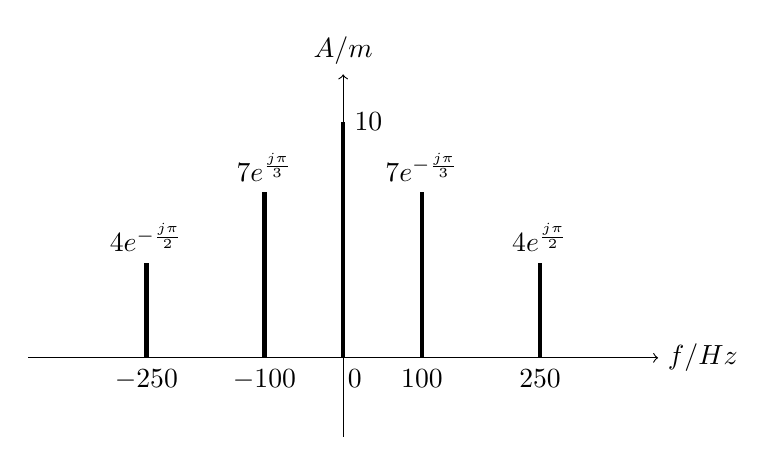
\begin{tikzpicture}
            \draw[->] (-4,0) -- (4,0) node[right] {$f/Hz$};
            \draw[->] (0,-1) -- (0,3.6) node[above] {$A/m$};
            \draw[ultra thick, black] (0,0) node[below] {$\;\;\;0$} -- (0,3) node[right] {$10$};
            \draw[ultra thick, black] (1,0) node[below] {$100$} -- (1,2.1) node[above] {$7e^{-\frac{j\pi}{3}}$};
            \draw[ultra thick, black] (2.5,0) node[below] {$250$} -- (2.5,1.2) node[above] {$4e^{\frac{j\pi}{2}}$};
            \draw[ultra thick, black] (-1,0) node[below] {$-100$} -- (-1,2.1) node[above] {$7e^{\frac{j\pi}{3}}$};
            \draw[ultra thick, black] (-2.5,0) node[below] {$-250$} -- (-2.5,1.2) node[above] {$4e^{-\frac{j\pi}{2}}$};
        \end{tikzpicture}
    \end{center}

    Multiplying something by $i$ jas an effect of rotating that something by 90 degrees. 
    Using euler's formula, we can express any unit-length complex number as $e ^ {(2 \pi i t)}$
    Where $t$ is a real number, if $t$ represents time, 
    and plot the location of the complexnumber at the given time $t$.
    What we will see is a circle being drawn with a frequency of one cycle per second($Hz$).
    We could adjust the speed of the rotation by multiplying a frequency $f$ to the power, 
    which gives us $e ^ {(2 \pi i f t)}$\\\indent

    Can it have negative frequencies? negative frequencies seems pretty abstract at first, 
    but once you start to understand the idea of drawing a circle in the anti-clockwise direction,
    you will soon realise that having negative frequencies simply implies rotating in the clockwise direction.\\\indent

    Multipying the circle by a function $f(t)$ would then suggest wrapping the function around the circle,
    By taking the mean, finding the center of mass of the wrapped signal, at different time t with an integral, we can plot a diagram of the spectrum.
    When it all lined up, there will be an obvious peak. where the center of mass is shiped the farthest away from the signal.\\\indent

    So the complex version of fourier integrals is:

    \begin{align}
        x_k &= \frac{1}{T_0} \int_{0}^{T_0} x(t) e^{-j 2 \pi f_0 kt}
    \end{align}

\section{Discrete Signals}
    \subsection{Aliasing}
    Aliasing in the context of signal processing is simply the same name of two signals. 
    When sampling a signal at a certain frequency, multiple signals at different frequency can produce the same signal
    For, example: $\hat{\omega} + 2\pi l$ and $2\pi l - \hat{\omega}$ are aliases of $\hat{\omega}$
    as they are different discrete times signals defining the same signal values
    \begin{center}
        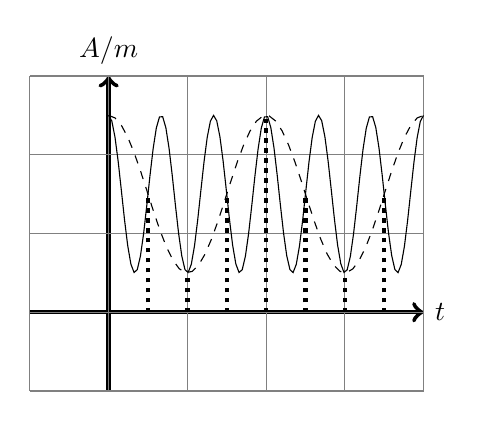
\begin{tikzpicture}
            \draw[->,ultra thick, black] (-1,0) -- (4,0) node[right] {$t$};
            \draw[->,ultra thick, black] (0,-1) -- (0,3) node[above] {$A/m$};
            \draw[gray] (-1,-1) grid (4,3);
            \draw [domain=0:4, samples=50,dashed] plot (\x, {1.5+cos(pi*\x r)});
            \draw [domain=0:4, samples=100] plot (\x, {1.5+cos(pi*\x*3 r)});
            \draw[dotted, ultra thick, black] (0.5,0) -- (0.5,1.5);
            \draw[dotted, ultra thick, black] (1.0,0) -- (1.0,0.5);
            \draw[dotted, ultra thick, black] (1.5,0) -- (1.5,1.5);
            \draw[dotted, ultra thick, black] (2.0,0) -- (2.0,2.5);
            \draw[dotted, ultra thick, black] (2.5,0) -- (2.5,1.5);
            \draw[dotted, ultra thick, black] (3.0,0) -- (3.0,0.5);
            \draw[dotted, ultra thick, black] (3.5,0) -- (3.5,1.5);
        \end{tikzpicture}
    \end{center}
    As you can see from the diagram above, the two signal, both sampled at 2 Hz, 
    produced the same value each sample, but are fundamentally, two different frequencies\\\indent

    The principle alias is the frequency in $[0, \pi]$

    \begin{align}
        \hat{\omega}\; &\hat{\equiv}\; \omega_0 T_s = \frac{\omega_0}{f_s}
    \end{align}

    Fix a discrete sinusioid of discrete-time frequency $\hat{\omega}$, then the frequency $f_0$ of the original continuous
    time sinusoid could have been any of the following:

    \begin{align}
        f_0 = (\frac{\hat{\omega}}{2\pi})f_S \;\text{or}\; f_0 = (\frac{\hat{\omega}}{2\pi})f_S + lf_s \;\text{or}\; f_0 =  lf_s - (\frac{\hat{\omega}}{2\pi})f_s \; where l \in \mathbb{Z}
    \end{align}

    We cannot know which one of them is the true signal, unless we can fix more conditions

    \subsubsection{Sampling sinusoids}

    Take a sample of $x[n] = cos(0.4 \pi n)$, and is equivalent to $x_2[n] = cos(2.4 \pi n)$. An alias corresponding to the principal alias , by convention, is used.
    Once the name is fixed and $f_s$ is known, we canguarantee that the samples came from 
    \begin{align}
        x[n] &=\; cos(0.4 \pi n) \;\text{since}\; \hat{\omega} \in [0,\pi] \\
        \implies \omega_0 &=  \hat{\omega} f_s \in [0,\pi \times f_s]\\
        \implies f_0 &= \frac{f_0}{2\pi} \in [0, \frac{f_s}{2}]
    \end{align}

    If the frequency of the original continuous time signal does not satisfy the condition mentioned above, 
    then the resulting samples are identical to those obtained by sampling a lower frequency signal. So When
    $f_0 \notin [0, \frac{f_s}{2}]$, aliasing occurs.

    Example:

    Continuous-time signal $x(t) = cos(2\pi (100) t)$ with sampling frequency $f_s = 500 Hz$. 

    \begin{center}
        \begin{tikzpicture}
            \draw[->] (-4,0) -- (4,0) node[right] {$f/Hz$};
            \draw[->] (0,-1) -- (0,3.6) node[above] {$A/m$};
            \draw[ultra thick, black] (2,0) node[below] {$100$} -- (2,2) node[right] {$0.5$};
            \draw[ultra thick, black] (-2,0) node[below] {$-100$} -- (-2,2) node[above] {$0.5$};
        \end{tikzpicture}
    \end{center}

    The signal is baud-limited where $f_{max} = 100 Hz$. 
    The sampling frequency is larger than the Nyquist rate$(2f_{max} = 200 Hz)$, so this is an over-sampling

    \begin{align}
        \hat{\omega} &= \frac{2\pi \times 100}{f_s} = 0.4\pi\\
        \hat{\omega} &= 0.4 \pi + 2\pi l\\
        \hat{\omega} &= 2\pi l - 0.4 \pi\\
        &\text{where} l \in \mathbb{Z} \nonumber
    \end{align}

    Hence the discrete-time spectrum plot looks like:
    \begin{center}
        \begin{tikzpicture}
            \draw[->] (-4,0) -- (4,0) node[right] {$\pi \hat{\omega} / rad$};
            \draw[->] (0,-1) -- (0,3.6) node[above] {$A/m$};
            \draw[ultra thick, black] (0.8,0) node[below] {$0.4$} -- (0.8,2) node[right] {$0.5$};
            \draw[ultra thick, black] (3.2,0) node[below] {$1.6$} -- (3.2,2) node[above] {$0.5$};
            \draw[ultra thick, black] (-0.8,0) node[below] {$-0.4$} -- (-0.8,2) node[right] {$0.5$};
            \draw[ultra thick, black] (-3.2,0) node[below] {$-1.6$} -- (-3.2,2) node[above] {$0.5$};
        \end{tikzpicture}
    \end{center}

    \subsection{Discrete to Continuous Converter}
    Disrete to Continuous Converter (D2C for short), interpolates a smooth Continuous function 
    through the given discrete samplesy[n].
    A special case is $y[n] = Acos(\hat{\omega} n + \phi)$ In ideal case, $y(t) = Acos(2\pi f_0 t + \phi)$
    should be produced. Only $f_0$ is required which can be found easily by $\hat{\omega}$.\newline\indent

    \noindent For more general signal, according to sampling theorem, we can still produce $y(t)$ as long as $f_s > 2f_{max}$

    \noindent A popular model is \newline\indent
    
    $s(t) = \sum_{n \in \mathbb{Z}}{s[n]p(t-nT_s)} where p(t) is a characteristic pulse of the converter$\newline\indent
    
    Weighting signal as linear combination of time-shifted pulses.

    \begin{center}
        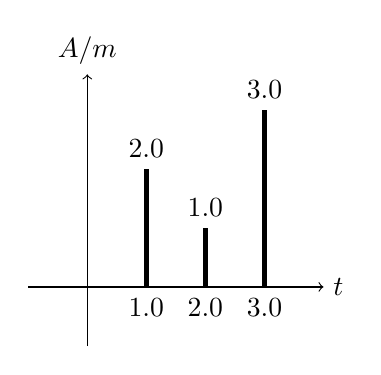
\begin{tikzpicture}[scale=0.75]
            \draw[->] (-1,0) -- (4,0) node[right] {$t$};
            \draw[->] (0,-1) -- (0,3.6) node[above] {$A/m$};
            \draw[ultra thick, black] (1,0) node[below] {$1.0$} -- (1,2) node[above] {$2.0$};
            \draw[ultra thick, black] (2,0) node[below] {$2.0$} -- (2,1) node[above] {$1.0$};
            \draw[ultra thick, black] (3,0) node[below] {$3.0$} -- (3,3) node[above] {$3.0$};
        \end{tikzpicture}
        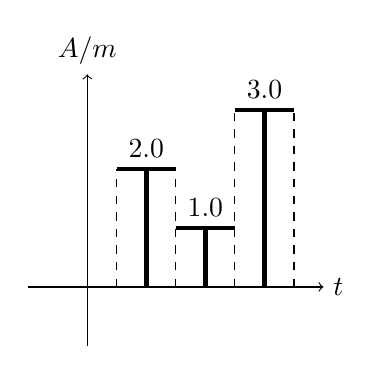
\begin{tikzpicture}[scale=0.75]
            \draw[->] (-1,0) -- (4,0) node[right] {$t$};
            \draw[->] (0,-1) -- (0,3.6) node[above] {$A/m$};
            \draw[dashed] (0.5,0) -- (0.5,2);
            \draw[ultra thick] (1,0) -- (1,2) node[above] {$2.0$};
            \draw[ultra thick, black] (0.5,2) -- (1.5,2);
            \draw[dashed] (1.5,0) -- (1.5,2);
            \draw[ultra thick] (2,0) -- (2,1) node[above] {$1.0$};
            \draw[ultra thick, black] (1.5,1) -- (2.5,1);
            \draw[dashed] (2.5,0) -- (2.5,3);
            \draw[ultra thick] (3,0) -- (3,3) node[above] {$3.0$};
            \draw[ultra thick, black] (2.5,3) -- (3.5,3);
            \draw[dashed] (3.5,0) -- (3.5,3);
        \end{tikzpicture}
    \end{center}

    If by linear interpolation
    \begin{center}
        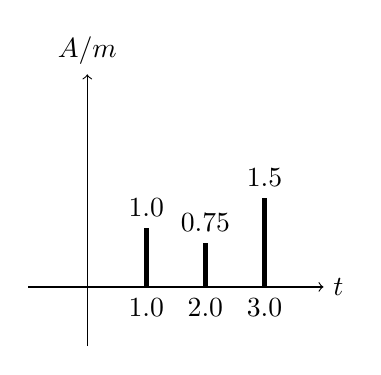
\begin{tikzpicture}[scale=0.75]
            \draw[->] (-1,0) -- (4,0) node[right] {$t$};
            \draw[->] (0,-1) -- (0,3.6) node[above] {$A/m$};
            \draw[ultra thick, black] (1,0) node[below] {$1.0$} -- (1,1.0) node[above] {$1.0$};
            \draw[ultra thick, black] (2,0) node[below] {$2.0$} -- (2,0.75) node[above] {$0.75$};
            \draw[ultra thick, black] (3,0) node[below] {$3.0$} -- (3,1.5) node[above] {$1.5$};
        \end{tikzpicture}
        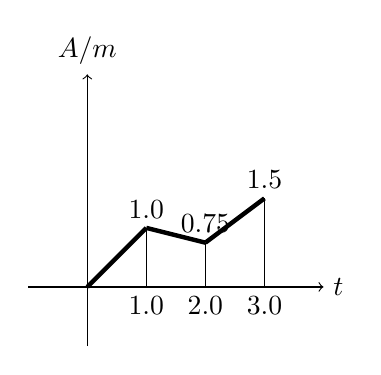
\begin{tikzpicture}[scale=0.75]
            \draw[->] (-1,0) -- (4,0) node[right] {$t$};
            \draw[->] (0,-1) -- (0,3.6) node[above] {$A/m$};
            \draw[ultra thick, black] (0,0) -- (1,1);
            \draw (1,0) node[below] {$1.0$} -- (1,1.0) node[above] {$1.0$};
            \draw[ultra thick, black] (1,1) -- (2,0.75);
            \draw (2,0) node[below] {$2.0$} -- (2,0.75) node[above] {$0.75$};
            \draw[ultra thick, black] (2,0.75) -- (3,1.5);
            \draw (3,0) node[below] {$3.0$} -- (3,1.5) node[above] {$1.5$};
        \end{tikzpicture}
    \end{center}

    Ideal Pulse:

    \begin{align}
        p(t) &= sin(\frac{t}{T_s}) = \frac{sin(\frac{nt}{T_s})}{\frac{nt}{T_s}}\;where\;t in \pm \infty\\
        p(n \times T_s) &= \frac{sin(\pi n)}{\pi n} =
        \begin{cases}
            1, & n=0\\
            0, & n = \pm 1, \pm 2, \dots
        \end{cases} 
    \end{align}

    \noindent Pulse has infinite length $\Rightarrow$ All samples are needed to reconstruct a signal exactly from its samples.

    Let $x[n] = cos(\hat{\omega}n+\phi)$, find $x_{out}(t)$ for the given sampling rates $f_s$
    \begin{align}
        &f_s = 500 Hz,\;\hat{\omega} = 0.4\pi\\
        &\hat{\omega} \in [0,\pi] \Rightarrow \hat{\omega_{p}} = \hat{\omega} = 0.4\pi\\
        &\omega_{out} = \hat{\omega} \times f_s = 0.4\pi \times 500 = 200\pi \Rightarrow f_{out} = 100Hz\\
        &\nonumber\\
        &f_s = 500 Hz,\;\hat{\omega} = 1.6\pi\\
        &\hat{\omega} \notin [0,\pi] \Rightarrow \hat{\omega_{p}} = 2\pi-\hat{\omega} = 0.4\pi\\
        &\omega_{out} = \hat{\omega} \times f_s = 0.4\pi \times 500 = 200\pi \Rightarrow f_{out} = 100Hz\\
        &\nonumber\\
        &f_s = 80 Hz,\;\hat{\omega} = 2.5\pi\\
        &\hat{\omega} \notin [0,\pi] \Rightarrow \hat{\omega_{p}} = 2\pi\hat{\omega} = 0.5\pi\\
        &\omega_{out} = \hat{\omega} \times f_s = 0.5\pi \times 80 = 40\pi \Rightarrow f_{out} = 20Hz\\
    \end{align}

\section{Brief introduction to Systems}
    \subsection{Filters}
    Generally a filter can be classified as Running-Average or FIR(Finite impulse response). 

    \noindent A Filter is a system designed to remove source components or modify some characteristic of a signal.\\\indent

    \noindent A discrete-time system is a computational process for transforming 
    one sequence in to another sequence (input to output)\\\indent

    Systems are often depicted as block diagram
    \begin{center}
        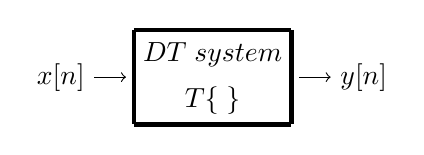
\begin{tikzpicture}
            \draw[->] (-1.5,0) node[left] {$x[n]$} -- (-1.1,0);
            \draw[->] (1.1,0) -- (1.5,0) node[right] {$y[n]$};
            \draw (0,0) node[above] {$DT\;system$} node[below] {$T\{\;\}$};
            \draw[ultra thick, black] (-1,0.6) -- (1,0.6);
            \draw[ultra thick, black] (-1,-0.6) -- (1,-0.6);
            \draw[ultra thick, black] (-1,0.6) -- (-1,-0.6);
            \draw[ultra thick, black] (1,0.6) -- (1,-0.6);
        \end{tikzpicture}
    \end{center}
    We seen D2C and C2D before, here we focus on systems where both input and output are discrete, 
    such systems can be implemented with digital computations.\\\indent

    \noindent Mathematical Representation:

    \noindent We represent the operation of a system by a operator $T\{\;\}$
    \begin{align}
        y[n] &= T\{x[n]\}\text{\; such as:\;}\\
        y[n] &= (x[n])^2\\
        y[n] &= \frac{\sum_{i = 0}^{i=2}{\{x[n-i]\}}}{2}
    \end{align}

    \noindent Running-Average Filters (RAF):\\\indent

    \noindent Infact (85) mentioned above, is an 3-point-RA system
    Consider a finite length signal $x[n]$ where $x[n]$ itself is defined only in $0~4$
    Apply a 3-point-RA system, $y[n] = \frac{\sum_{i = 0}^{i=2}{\{x[n+i]\}}}{3}$ to it

    \begin{center}
        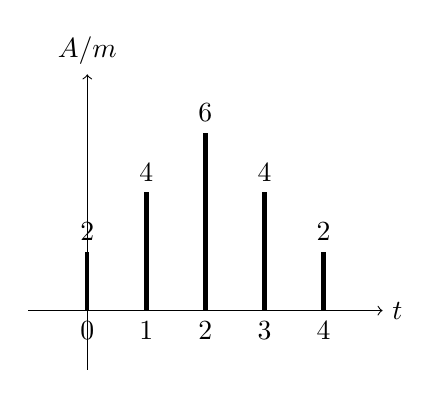
\begin{tikzpicture}[scale = 0.75]
            \draw[->] (-1,0) -- (5,0) node[right] {$t$};
            \draw[->] (0,-1) -- (0,4) node[above] {$A/m$};
            \draw[ultra thick, black] (0,0) node[below] {$0$} -- (0,1)node[above] {$2$};
            \draw[ultra thick, black] (1,0) node[below] {$1$} -- (1,2)node[above] {$4$};
            \draw[ultra thick, black] (2,0) node[below] {$2$} -- (2,3)node[above] {$6$};
            \draw[ultra thick, black] (3,0) node[below] {$3$} -- (3,2)node[above] {$4$};
            \draw[ultra thick, black] (4,0) node[below] {$4$} -- (4,1)node[above] {$2$};
        \end{tikzpicture}
        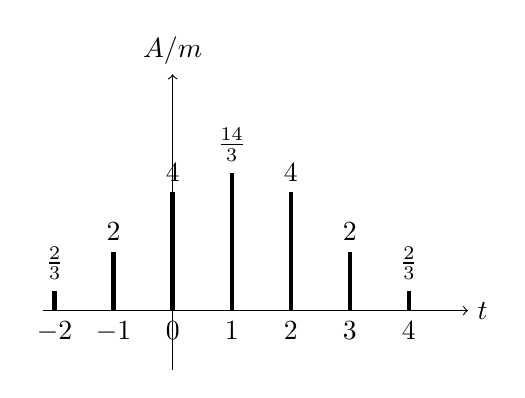
\begin{tikzpicture}[scale = 0.75]
            \draw[->] (-2.2,0) -- (5,0) node[right] {$t$};
            \draw[->] (0,-1) -- (0,4) node[above] {$A/m$};
            \draw[ultra thick, black] (-2,0) node[below] {$-2$} -- (-2,1/3)node[above] {$\frac{2}{3}$};
            \draw[ultra thick, black] (-1,0) node[below] {$-1$} -- (-1,1)node[above] {$2$};
            \draw[ultra thick, black] (0,0) node[below] {$0$} -- (0,2)node[above] {$4$};
            \draw[ultra thick, black] (1,0) node[below] {$1$} -- (1,7/3)node[above] {$\frac{14}{3}$};
            \draw[ultra thick, black] (2,0) node[below] {$2$} -- (2,2)node[above] {$4$};
            \draw[ultra thick, black] (3,0) node[below] {$3$} -- (3,1)node[above] {$2$};
            \draw[ultra thick, black] (4,0) node[below] {$4$} -- (4,1/3)node[above] {$\frac{2}{3}$};
        \end{tikzpicture}
    \end{center}
    The output still has finite support and is longer, and it starts before the input starts. It uses the future values so it is a non-causal system

    \noindent Causal means that the filter uses only the present and past values of the input. 
    Non-causals are not implemented in real-time as future signal is not possible to obtain,
    but can be used in stored data.
    \begin{align}
        y[n] &= \frac{\sum_{i = 0}^{i=2}{\{x[nii]\}}}{3}\;or\\
        y[n] &= \frac{\sum_{l = n-2}^{n}{\{x[n]\}}}{3}\;or\\
        y[n] &= y[n-1] + 1/3(x[n] - x[n-3])
    \end{align}
    would be an causal RAF

    \noindent If the length of x[n] is N, 
    the length of the output of RAF after running through an M point RAF would be
    $N + M - 1$

    \noindent Take an uncorrupted signal vector $s$, random noise $z^{i}$ and a measurement result $x^{i}$,
    $x^{i} = s + z^{i}$, the ensemble average after k measurements is given by:

    \begin{align}
        x_{ave}[n] &= \frac{1}{k}\sum_{i=0}^{k}x^{i}[n]\\ 
                   &= s[n] + \frac{1}{k}\sum_{i=0}^{k}z^{i}[n]
    \end{align}

    The $\frac{1}{k}\sum_{i=0}^{k}z^{i}[n]$ part is usually very small for random noise. 
    The ensemble average gives a good estimate of the uncorrupte data over a large number of measurements k.
    If the data being measured cannot be repeated, then simply averaging a set of consecutive measurements
    often provides a reasonable estimate of the uncorrupted data.\\\indent

    \noindent An FIR filter is similar, but for each there's a certain coefficient determined by the position.
    $y[n] = \frac{1}{k}\sum_{l=0}^{M}{h_l \times x[n-l]}$, where $h_l$ is one of the number in array 
    $\{h_0,h_1,h_2,\dots,h_M\}$ this takes no future values, so it is a causal system. 
    If we take the array as another signal, we can have the relationship 
    $y[n] = \frac{1}{k}\sum_{l=0}^{M}{h[l] \times x[n-l]}$, which is called convolution sum.\\\indent

    \subsubsection{Linearity}

    \noindent If a system is linear, then if splitting the input into linear combination of two other functions
    and run them through the system seperately. We should get the same result as running the original system through it. 
    So $y[n] = |x[n]|$ is obviously not an linear system.\\\indent

    \noindent Mathematically, we denote the process as this:
    \begin{align}
        Let x[n] &= \alpha x_1[n] + \beta x_2[n]
        T\{\alpha x_1[n] + \beta x_2[n]\} &= \alpha T\{x_1[n]\} + \beta T\{x_2[n]\}
    \end{align}

    \subsubsection{Time-Invariant}
    If a input is delayed and as a response the output is delayed by the same amount,
    We said that it is a Time-Invariant system. 
    Take Delayed input response $y_1[n]$ and Delayed-Output-Response$y[n-\phi]$
    \begin{align}
        Let\; y[n] &= \alpha x[n] \\
        y_1[n] &= \alpha x[n - \phi] \\
        y[n - \phi] &= \alpha x[n - \phi]\\
        y_1[n] &\equiv y[n - \phi]
    \end{align}
    So the system is Time-Invariant.
    \begin{align}
        Let\; y[n] &= n \times x[n] \\
        y_1[n] &= (n)\times x[n - \phi] \\
        y[n - \phi] &= (n - \phi)\times x[n - \phi]\\
        y_1[n] &\not\equiv y[n - \phi]
    \end{align}
    So the system is not Time-Invariant (Time-Variant)\\\indent

    Turns out, Impulse response is a complete characteristic of any Linear Time Invariant System\\\indent

    There used to be many form of communications: such as telegraphy, video and so on. 
    They are all developed independently, with different methods of communication.
    As the network grew bigger they need a way to combine so they can work together.
    This increased focus on underlying principles of communication systems.
    Bell laboratories at AT\&T back in the 1910s to 50s were the center of the most important developments.
    In 1948 Claude Shannon published his work "A mathematical theory of communication", 
    which in a way created the Information Theory.\\\indent

    Shannon introduced a model that didn't depoend on a particular system or technology,
    As shown in the diagram below.

    \begin{center}
        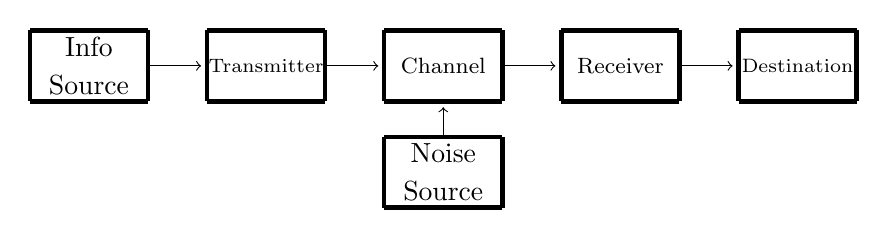
\begin{tikzpicture}[scale = 0.75]

            \draw[ultra thick] (-1,-1.2) -- (1,-1.2) (-1,-2.4) -- (1,-2.4) (-1,-1.2) -- (-1,-2.4) (1,-1.2) -- (1,-2.4);
            \draw (0,-1.8) node[above] {Noise} node[below] {Source};
            \draw[->] (0,-1.2) -- (0,-0.7);

            \draw[ultra thick] (-5,0.6) -- (-7,0.6) (-5,-0.6) -- (-7,-0.6) (-5,0.6) -- (-5,-0.6) (-7,0.6) -- (-7,-0.6);
            \draw (-6,0) node[above] {Info} node[below] {Source};
            \draw[->] (-5,0) -- (-4.1,0);

            \draw[ultra thick] (-4,0.6) -- (-2,0.6) (-4,-0.6) -- (-2,-0.6) (-4,0.6) -- (-4,-0.6) (-2,0.6) -- (-2,-0.6);
            \draw (-3,0) node {\scriptsize Transmitter};
            \draw[->] (-2,0) -- (-1.1,0);

            \draw[ultra thick] (-1,0.6) -- (1,0.6) (-1,-0.6) -- (1,-0.6) (-1,0.6) -- (-1,-0.6) (1,0.6) -- (1,-0.6);
            \draw (0,0) node {\footnotesize Channel};
            \draw[->] (1,0) -- (1.9,0);

            \draw[ultra thick] (4,0.6) -- (2,0.6) (4,-0.6) -- (2,-0.6) (2,0.6) -- (2,-0.6) (4,0.6) -- (4,-0.6);
            \draw (3,0) node {\footnotesize Receiver};
            \draw[->] (4,0) -- (4.9,0);

            \draw[ultra thick] (5,0.6) -- (7,0.6) (5,-0.6) -- (7,-0.6) (5,0.6) -- (5,-0.6) (7,0.6) -- (7,-0.6);
            \draw (6,0) node {\scriptsize Destination};
        \end{tikzpicture}
    \end{center}
    Now clear questions can be raised about any syetem.
    \begin{enumerate}
        \item How much information does a source produce?
        \item What is the best way to encode a message in the transmitter?
        \item Is there a limit to the amount of info we can send over the Channel
        \item How badly noise affects the transmission?
        \item How to model different communication sourses?
        \item How to measure information?
    \end{enumerate}

    Source might be discrete(letters, binary numbers) or analog(voltage, amplitude).
    All communication sources can be represented by binary sequences. 
    The output of the source, instead of waiting for a certain input, is modeled as random.
    The idea of applying an ADC was revolutionary in 1948. \\\indent

    One of the simplest information source is just tossing a coin with two outcome with equal possibilities.
    We can use 0 and 1 to record the information, so only one bit is needed. 
    If the coin is unfair and we can only gain 0, no bit (0 bit) is needed.\\\indent

    According to shannom, information is a measure of uncertainty. 
    Hence the information of a source is a measurement of the average uncertainty in the outcome of the source.
    If we have a source of output with 256 possible symbol, how many bits do we need to send one?\\\indent

    We could use 256 bits which is 32 byte of data, which in today's standard is pretty small.
    But it is a gigantic amount of data back then (even for some systems today it is still pretty big).
    Since $log_{2}(256) = 8$, all we need is 1 byte(8 bit) of data.\\\indent

    Suppose we have a horse race with 8 houses each with integer number $n \in [0,7]$, with winning chances
    \begin{align}
        P(N = n) = 
        \begin{cases}
            \frac{1}{2^{(n+1)}} n \in [0,3]\\
            \frac{1}{2} n >= 4\\
        \end{cases} 
    \end{align}
    How many bits do we need? We could use 1 byte of data, 
    or we could use 3 bits of data if we need to save some space.
    Can we do even better then this? 
    Well, if we model the length of the bits we used like another model, 
    and find the expected length ($E(l)$) of data, we might be able to do even better.
    \begin{align}
        Length(data) &= 
        \begin{cases}
            n + 1,\;n \in [0,3]\\
            6,\;n >= 4\\
        \end{cases}\\
        E(l) &= \sum_{i = 0}^{3}{\biggr\{\frac{1}{2^(i+1)} \times (i+1)\biggr\}} + \frac{1}{64} \times 6\\
             &= 2
    \end{align}
    Average bit length = 2, so we should be able to use 2 bits to model the entire thing, which should be enough.
    The way we calculated the expected length, is called the \underline{entropy} of the source.
    \begin{align}
        H &= -\sum_{i = 1}^{N}{(P(i)\times log_2(P(i)))}\\
        \text{Entropy of free coin~} P1 = P2 &= 0.5\\
        H &= -0.5\;log_2(0.5) + -0.5\;log_2(0.5)\\
          &= (-0.5 \times -1) + (-0.5 \times -1)\\
          &= 0.5 + 0.5\\
          &= 1
    \end{align}
    In an informal way, Entropy is a lower bound of the average number of bits required to represent the random variable.
    \newpage
\section{Review}
    \subsection{Signals}
        Signals are patterns of variation that represent or encode information.
            \begin{enumerate}
                \item They are mathematically represented as a function of one or more variables
                \item Continuous Variable $\rightarrow$ Continuous Signals \\ 
                      Discrete Variable $\rightarrow$ Discrete Signals
            \end{enumerate}
            \begin{center}
                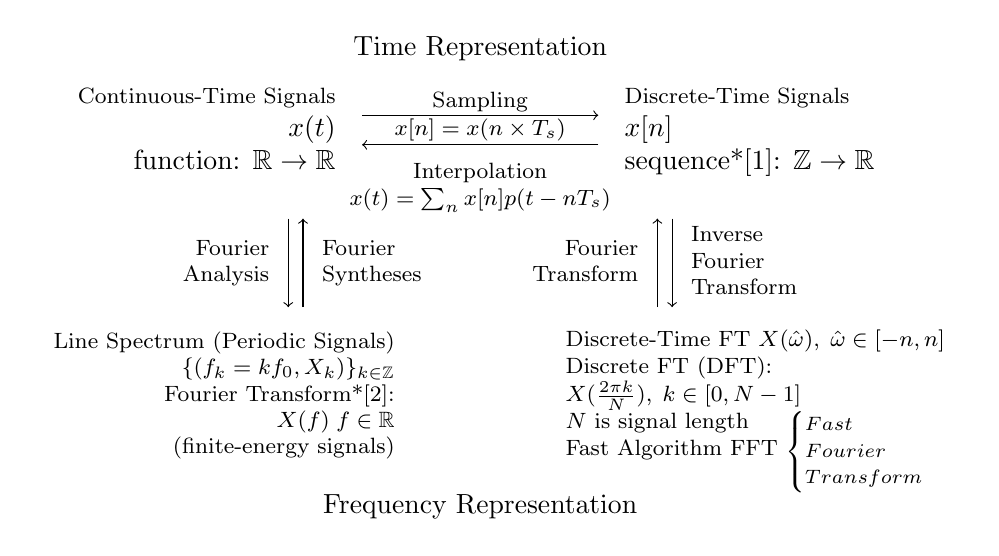
\begin{tikzpicture}[scale = 0.75]
                    \draw (0,3) node[above] {Time Representation};
                    \draw[->] (-2,2.25) -- (2,2.25);
                    \draw (0,2.15) node[above] {\footnotesize{Sampling}} (0,2.35) node[below] {\footnotesize{$x[n] = x(n \times T_s)$}};
                    \draw[->] (2,1.75) node[left] {} -- (-2,1.75) node[right] {};
                    \draw (0,1.65) node[below] {\footnotesize \begin{tabular}{c} Interpolation \\ $x(t) = \sum_n{x[n]p(t-nT_s)}$ \end{tabular}};
                    \draw[] (-2, 2) node[left] {\begin{tabular}{r} \footnotesize{Continuous-Time Signals} \\ $x(t)$ \\ function: $\mathbb{R}\rightarrow\mathbb{R}$ \end{tabular}}
                            (2,2) node[right] {\begin{tabular}{l} \footnotesize{Discrete-Time Signals} \\ $x[n]$ \\ sequence*[1]: $\mathbb{Z}\rightarrow\mathbb{R}$ \end{tabular}};

                    \draw[->] (-3,-1) -- (-3,0.5);
                    \draw[] (-3.125,-0.25) node[left]{\footnotesize\begin{tabular}{r} Fourier\\Analysis\end{tabular}}
                         node[right]{\footnotesize\begin{tabular}{l} Fourier\\Syntheses\end{tabular}};
                    \draw[->] (-3.25,0.5) -- (-3.25,-1);

                    \draw[->] (3,-1) -- (3,0.5);
                    \draw[] (3.125,-0.25) node[left]{\footnotesize\begin{tabular}{r} Fourier\\Transform\end{tabular}}
                         node[right]{\footnotesize\begin{tabular}{l} Inverse\\Fourier\\Transform\end{tabular}};
                    \draw[->] (3.25,0.5) -- (3.25,-1);

                    \draw (0,-4) node[below] {Frequency Representation};
                    \draw[] (-1, -2.5) node[left] {\footnotesize\begin{tabular}{r}
                                Line Spectrum (Periodic Signals) \\
                                $\{(f_k = k f_0, X_k)\}_{k\in\mathbb{Z}}$\\
                                Fourier Transform*[2]:\\
                                $X(f)\; f \in \mathbb{R}$\\
                                (finite-energy signals)
                            \end{tabular}}
                            (1,-2.5) node[right] {\footnotesize\begin{tabular}{l}
                                Discrete-Time FT $X(\hat{\omega}),\;\hat{\omega}\in[-n,n]$ \\ 
                                Discrete FT (DFT):\\ 
                                $X(\frac{2\pi k}{N}),\;k\in[0,N-1]$\\
                                $N$ is signal length\\
                                Fast Algorithm FFT
                            \end{tabular}}
                        (5,-3.45) node[right] {\scriptsize$\begin{cases}Fast\\Fourier\\Transform\end{cases}$};

                    \draw[] (4,2) node[right] {};
                    \draw[] (4,-2) node[below]{};
                    \draw[] (-4,-2) node[below]{};
                \end{tikzpicture}
            \end{center}
            [1] Digital Signals only take finite number of values, we ignore qualization in this course

            [2] We did not cover the continuous-time Fourier Transformation, 
            it will be introduced at a high-level in the future as a generalization of the line-spectrum for non-periodic signals
    \subsection{Fourier Series}
        Any periodic real signals (which can be proven by) $x(t) = x(t + \frac{1}{f_0})$ 
        can be written as a (possibly infinite) amount of addictive linear combination of (complex) sinusoidal signals:
        \small{\begin{align}
            x(t)&= X_0 + \sum_{k = 1}^{+\infty}{X_k e^{2\pi i\times f_0 k t} + X_k* e^{-2k\pi i\times f_0 t}}\\
                &= \sum_{k = -\infty}^{\infty}{X_k e^{2\pi i\times f_0 k t}} (X_{-k} = X*_{k})\\
                &\equiv x(t) = A_0 + \sum_{k = 1}^{+\infty}{A_kcos(2\pi f_0kt + \phi_k)}\\
                &\text{Where}\; X_0 = A_0\;\text{and}\;X_k = \frac{1}{2} A_k e^{i\Phi k} \nonumber
        \end{align}}
            \subsubsection{Line Spectrum}
            The set of pairs:
            $\{\dots,(-f_k, \frac{1}{2}X_k*),\dots,(-f, \frac{1}{2}X_1*),(0,X_0),(f_1, \frac{1}{2}X_1),\dots,(f_k, \frac{1}{2}X_k)\}$
            \textbf{(Why Fourier Representation?)}
            \renewcommand{\labelitemi}{\textendash}
            \begin{enumerate}
                \item Can reveal information about the signal that is not easy to spot 
                in the time-domain representation\textit{[Refer to "Finding a note"]}
                \item As such, it helps identify structure/properties of the signal
                \item These properties can be used later as information that helps processing a signal
                \item For example, cans use Fourier representation for denoising:
                    \begin{itemize}
                        \item
                        Idea is that noise usually has high-frequencies that are "separated" from
                        the useful frequencies of the signal, so denoising can be done in frequency
                        domain\textit{[Refer to "Noise-Filtering-Solutions"]} in ThinkDSP
                    \end{itemize}
                \item Can also use to compress a signal
                    \begin{itemize}
                        \item
                        Idea is only to use dominant frequencies (i.e. Frequencies with large magnitude)
                        \textit{[Recall the square wave approximation]}
                    \end{itemize}
                \item The input-output relation of an LTI(Linear-Time-Invariant) system is simpler to view in
                Frequency domain as is a simple multiplication
                    \begin{itemize}
                        \item Algorithmic gain can gain easier infuition about about filter operations
                        \item Computational gain: fast way to perform convolution thanks to numpy's FFT
                    \end{itemize}
            \end{enumerate}
            \renewcommand{\labelitemi}{\textbullet}
            
            \textbf{Fourier Synthesis}
                \begin{align}
                    \sum_{-\infty}^{\infty}{X_k e^(2\pi i f_0 k T)}
                \end{align}
            \textbf{Fourier Analysis}
                \begin{align}
                    X_k = \frac{1}{T_0}\int_{\frac{T_0}{2}}^{-\frac{T_0}{2}}{x(t)e^(-2\pi i f_0 k T)}
                \end{align}
            \textbf{Complex Amplitude}
                $X_k\leftarrow$ Complex Numbers
                \renewcommand{\labelitemi}{\textendash}
                \begin{itemize}
                    \item Magnitude $|X_k|$
                    \item Phase $arg(X_k)$
                    \item Polar Form: $X_k = |X_k|e^(iarg(X_k))$
                \end{itemize}
                Recall Euler's Formula:
                \begin{align}
                    e^{i\theta} &= cos(\theta) + isin(\theta)\\
                    cos(\theta) = \Re(z) &= \frac{1}{2} (z+z*) = \frac{1}{2}(e^{i\theta} + e^{-i\theta})\\
                    sin(\theta) = \Im(z)&= \frac{1}{2i}(z-z*) = \frac{1}{2i}(e^{i\theta} - e^{-i\theta})
                \end{align}
                \renewcommand{\labelitemi}{\textbullet}
    \subsection{Sampling}
            $x[n] = x(nT_s) = x[n\frac{1}{f_s}]$ \dots of sinusoids
            \begin{align}
                x(t) &= cos(2 \pi f_0 t + \Phi)\\
                \Rightarrow x[n] &= cos(\frac{\omega_0}{f_s}n + \Phi)~|~\omega_0 = 2\pi f_0\\
                &\overset{\mathrm{\Delta}}{=} cos(\hat{\omega}n + \Phi)~|~
                    \hat{\omega} \overset{\mathrm{\Delta}}{=} \frac{\omega_0}{f_s} = \omega_0 T_s
            \end{align}
            Where thelast one is normalized radian Discrete-Time Frequency
                \subsubsection{Aliasing}
                \begin{align}
                    cos(\hat{\omega}n + \Phi) = cos((2\pi l\pm\hat{\omega})n + \Phi)
                \end{align}
                    Infinite number of discretie-time signals can define the same values
                \begin{align}
                    \hat{\omega},~2\pi l + \hat{\omega},~2\pi l - \hat{\omega}~\text{aliases}
                \end{align}
                    So we defined that the principal alias is the frequency in [0,n]
                \subsubsection{Interpolation}
                By convention use the alias corresponding to the principal alias, principal alalias
                \begin{align}
                    \hat{\omega}\in[0,\pi]\Rightarrow \omega\in[0,\pi f_s] \Rightarrow f_0\in[0,\frac{f_s}{2}]
                \end{align}
                If original frequency not in $[0,\frac{f_s}{2}]$, then aliasing occurs. 
                Recall the sampling theorem, $f_s \geq 2f_{max}$

                A cut-time signal with frequencies no higher than $f_{max}$ can be reconstructed exactly from
                its samples $x[n] = x(nT_s)$ provided that the sampling rate $f_s = 1/T_s$ satisfies $f_s > 2f_{max}$
                where $2f_{max}$ is the Nyquist rate

                How reconstruction works:
                \begin{align}
                    x(t) = \sum_{n\in\mathbb{Z}} x[n]p(t-nT_s)
                \end{align}
                Ideal pulse:
                \begin{align}
                    p(t) = sinc(\frac{t}{T_s}) = \frac{sin(\frac{nt}{Ts})}{\frac{nt}{T_s}}
                \end{align}
                Practical Pulses: Zero-order hold Linear Interpolation
                \begin{center}
                    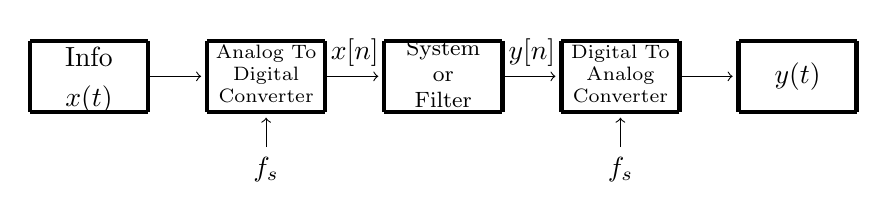
\begin{tikzpicture}[scale = 0.75]
            
                        \draw[ultra thick] (-5,0.6) -- (-7,0.6) (-5,-0.6) -- (-7,-0.6) (-5,0.6) -- (-5,-0.6) (-7,0.6) -- (-7,-0.6);
                        \draw (-6,0) node[above] {Info} node[below] {$x(t)$};
                        \draw[->] (-5,0) -- (-4.1,0);
            
                        \draw[ultra thick] (-4,0.6) -- (-2,0.6) (-4,-0.6) -- (-2,-0.6) (-4,0.6) -- (-4,-0.6) (-2,0.6) -- (-2,-0.6);
                        \draw (-3,0) node {\scriptsize \begin{tabular}{c}Analog To\\Digital\\Converter\end{tabular}};
                        \draw[->] (-3,-1.2) node[below]{$f_s$} -- (-3,-0.7);
                        \draw[->] (-2,0) -- (-1.1,0);

                        \draw (-1.5,0) node[above]{$x[n]$};
            
                        \draw[ultra thick] (-1,0.6) -- (1,0.6) (-1,-0.6) -- (1,-0.6) (-1,0.6) -- (-1,-0.6) (1,0.6) -- (1,-0.6);
                        \draw (0,0) node {\footnotesize \begin{tabular}{c}System\\or\\Filter\end{tabular}};
                        \draw[->] (1,0) -- (1.9,0);

                        \draw (1.5,0) node[above]{$y[n]$};
            
                        \draw[ultra thick] (4,0.6) -- (2,0.6) (4,-0.6) -- (2,-0.6) (2,0.6) -- (2,-0.6) (4,0.6) -- (4,-0.6);
                        \draw (3,0) node {\scriptsize \begin{tabular}{c}Digital To\\Analog\\Converter\end{tabular}};
                        \draw[->] (3,-1.2) node[below]{$f_s$} -- (3,-0.7);
                        \draw[->] (4,0) -- (4.9,0);
            
                        \draw[ultra thick] (5,0.6) -- (7,0.6) (5,-0.6) -- (7,-0.6) (5,0.6) -- (5,-0.6) (7,0.6) -- (7,-0.6);
                        \draw (6,0) node {$y(t)$};
                    \end{tikzpicture}
                \end{center}
    \subsection{Linear Time-Invariant Filters (LIT)}
        Fully characterized by their impulse-response $h[n]$ and the output to any input signal 
        $x[n]$ is the convolution of the input with the impulse response
        \begin{align}
            y[n] = h[n] * x[n]
        \end{align}
        \textbf{Focus}: FIR filters and finite-length inputsignals
        \begin{align}
            y[n] = \sum_{k = 0}^{M} {h[k]x[n-k]}
        \end{align}
        \textbf{Support set of the output}: 0,1,\dots,N+M-1
        \begin{align}
            \sigma[n] \rightarrow &\text{FIR} \rightarrow h[n] \nonumber\\
            x[n] \rightarrow &\text{FIR} \rightarrow y[n] = x[n] * h[n] \nonumber
        \end{align}
        \textbf{Key Idea}

        This way, we can view filters as signals, specifically LIT systems as their impulse response.
        $\Rightarrow$Can talk about frequency response of an LIT filter, 
        i.e. Frequency representation of its impulse response\\\indent

        \textbf{Fastway to perform convolution via FFT}
        \begin{align}
            y[n] = h[n]*x[n] \iff Y[k] = H[K] X[K]
        \end{align}
        In the above equation, $Y[k],~ H[K],~\text{and}~X[K]$ are Discrete Fourier Transform coefficients.\\\indent
        Convolution in time domain is multiplication in frequency domain.\\\indent

        \textbf{Examples}, Use of moving-averate filter for:
        \begin{enumerate}
            \item Smoothening: get rid of oscillations to reveal a trend
            \item Denoising: get rid of zero-mean random noise
        \end{enumerate}
        \begin{center}
            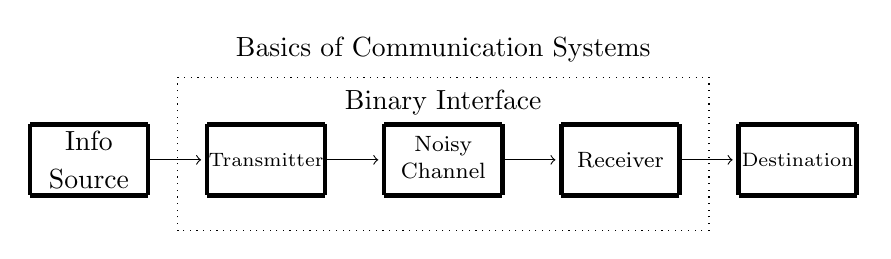
\begin{tikzpicture}[scale = 0.75]
            
                \draw[ultra thick] (-5,0.6) -- (-7,0.6) (-5,-0.6) -- (-7,-0.6) (-5,0.6) -- (-5,-0.6) (-7,0.6) -- (-7,-0.6);
                \draw (-6,0) node[above] {Info} node[below] {Source};
                \draw[->] (-5,0) -- (-4.1,0);
            
                \draw[ultra thick] (-4,0.6) -- (-2,0.6) (-4,-0.6) -- (-2,-0.6) (-4,0.6) -- (-4,-0.6) (-2,0.6) -- (-2,-0.6);
                \draw (-3,0) node {\scriptsize Transmitter};
                \draw[->] (-2,0) -- (-1.1,0);
            
                \draw[ultra thick] (-1,0.6) -- (1,0.6) (-1,-0.6) -- (1,-0.6) (-1,0.6) -- (-1,-0.6) (1,0.6) -- (1,-0.6);
                \draw (0,0) node {\footnotesize \begin{tabular}{c} Noisy \\ Channel \end{tabular}};
                \draw (0,0.6) node[above] {Binary Interface};
                \draw[->] (1,0) -- (1.9,0);
            
                \draw[ultra thick] (4,0.6) -- (2,0.6) (4,-0.6) -- (2,-0.6) (2,0.6) -- (2,-0.6) (4,0.6) -- (4,-0.6);
                \draw (3,0) node {\footnotesize Receiver};
                \draw[->] (4,0) -- (4.9,0);
            
                \draw[ultra thick] (5,0.6) -- (7,0.6) (5,-0.6) -- (7,-0.6) (5,0.6) -- (5,-0.6) (7,0.6) -- (7,-0.6);
                \draw (6,0) node {\scriptsize Destination};

                \draw[dotted](-4.5,-1.2) -- (-4.5,1.4) (4.5,-1.2) -- (4.5,1.4) (4.5,-1.2) -- (-4.5,-1.2) (-4.5,1.4) -- (4.5,1.4);
                \draw (0,1.5) node[above] {Basics of Communication Systems};
            \end{tikzpicture}
        \end{center}
        \textbf{Fundamental Questions}
        \begin{enumerate}
            \item Smoothening: get rid of oscillations to reveal a trend
            \item Denoising: get rid of zero-mean random noise
        \end{enumerate}
        Or can we achieve vanishing probs of error at a non trival(ie non zero) rate of communication\\\indent
        \textbf{Question 1:}
        How to measure information of a data source?\\\indent
        Model data sources as a stochastic process/signal. 
        One of the simplest such model is the output of the data source is 
        a discrete random variable X with probability mass function $P_x(x)$\\\indent
        Everyout is an independent relation of the Random variables
        x (next symbol is independent of previous variables)\\\indent

        [Shannon] Information of such a source is measured by the entropy of X:
        \begin{align}
            H(x) = \sum_{x \in A_x} {P(x)\times log_2(\frac{1}{2P(x)})}
        \end{align}
        Entropy is a measure of uncertainty about the outcome of the source.\\\indent
        \textbf{How to compress information?}
        \begin{enumerate}
            \item Use binary codes, it, to each possible source outcome assign a binary sequence (aka codeword).
            \item The length of each codeword can depend on the probability of the corresponding symbol.
            \item Goal is to design "Good" codes of minimum average length.
            \item "Good" codes are instantaneous (Self-Punctuating) codes.
            \item The limit of how small the minimum average length of an instanteous code can be , is entropy of the source
        \end{enumerate}
        \begin{align}
            L(C) \geq H(X)
        \end{align}
        For Python Parts:
        \begin{enumerate}[label=(\alph*)]
            \item If/Else statements
            \item For Loops
            \item functions
            \item Numpy Arrays
        \end{enumerate}
\end{document}